% questions.tex —— 2006 年·北京卷·理科 · 题目内容片段（无答案）
% 由 tools/generate_projects.py 依来源总账自 2006/2006_数学真题_北京理_试题.md 生成，勿手改（改源 MD 后重跑）


\begin{gktip}
\textbf{来源边界}：题签依据固定 PDF 首页照录。题面按固定 PDF 第1—2页转录，印刷页码为280—281。该固定副本的发布者、出版者、版次、来源链及官方身份均未核实；\texttt{ready} 仅为来源清单中的文件状态，不代表来源认证。固定 PDF 可见范围未见答案、解析、评分或总分。
\end{gktip}

\gkpart{一、选择题}

\begin{gktip}
以下第1页（印刷页280）含第1—8题。
\end{gktip}

\begin{question}
\gkti{1}在复平面内，复数 $\dfrac{1+i}{i}$ 对应的点位于\mbox{（　　）}。

（A）第一象限　　（B）第二象限　　（C）第三象限　　（D）第四象限

\end{question}
\begin{question}
\gkti{2}若 $\vec a$ 与 $\vec b-\vec c$ 都是非零向量，则“$\vec a\cdot\vec b=\vec a\cdot\vec c$”是“$\vec a\perp(\vec b-\vec c)$”的\mbox{（　　）}。

（A）充分而不必要条件　　（B）必要而不充分条件

（C）充分必要条件　　（D）既不充分也不必要条件

\end{question}
\begin{question}
\gkti{3}在 $1,2,3,4,5$ 这五个数字组成的没有重复数字的三位数中，各位数字之和为奇数的共有\mbox{（　　）}。

（A）36个　　（B）24个　　（C）18个　　（D）6个

\end{question}
\begin{question}
\gkti{4}平面 $\alpha$ 的斜线 $AB$ 交 $\alpha$ 于点 $B$，过定点 $A$ 的动直线 $l$ 与 $AB$ 垂直，且交 $\alpha$ 于点 $C$，则动点 $C$ 的轨迹是\mbox{（　　）}。

（A）一条直线　　（B）一个圆　　（C）一个椭圆　　（D）双曲线的一支

\end{question}
\begin{question}
\gkti{5}已知
\nopagebreak[4]
\[
f(x)=\begin{cases}
(3a-1)x+4a, & x<1,\\
\log_a x, & x\ge 1,
\end{cases}
\]
是 $(-\infty,+\infty)$ 上的减函数，那么 $a$ 的取值范围是\mbox{（　　）}。

（A）$(0,1)$　　（B）$\left(0,\dfrac13\right)$

（C）$\left[\dfrac17,\dfrac13\right)$　　（D）$\left[\dfrac17,1\right)$

\end{question}
\begin{question}
\gkti{6}在下列四个函数中，满足性质“对于区间 $(1,2)$ 上的任意 $x_1,x_2$（$x_1\ne x_2$），$|f(x_1)-f(x_2)|<|x_2-x_1|$ 恒成立”的只有\mbox{（　　）}。

（A）$f(x)=\dfrac1x$　　（B）$f(x)=|x|$　　（C）$f(x)=2^x$　　（D）$f(x)=x^2$

\end{question}
\begin{question}
\gkti{7}设
\nopagebreak[4]
\[
f(n)=2+2^4+2^7+2^{10}+\cdots+2^{3n+10}\quad(n\in\mathbb N),
\]
则 $f(n)$ 等于\mbox{（　　）}。

（A）$\dfrac27(8^n-1)$　　（B）$\dfrac27(8^{n+1}-1)$

（C）$\dfrac27(8^{n+3}-1)$　　（D）$\dfrac27(8^{n+4}-1)$

\Needspace{0.4\textheight}
\end{question}
\begin{question}
\gkti{8}如图为某三岔路口交通环岛的简化模型。在某高峰时段，单位时间进出路口 $A,B,C,$ 的机动车辆数如图所示，图中 $x_1,x_2,x_3$ 分别表示该时段单位时间通过路段 $\widehat{AB},\widehat{BC},\widehat{CA}$ 的机动车辆数（假设：单位时间内，在上述路段中，同一路段上驶入与驶出的车辆数相等），则 $x_1,x_2,x_3$ 的大小关系是\mbox{（　　）}。
\nopagebreak[4]
\begin{center}% Q8: 按固定候选 PDF 第1页（印刷页280）交通环岛图重绘。
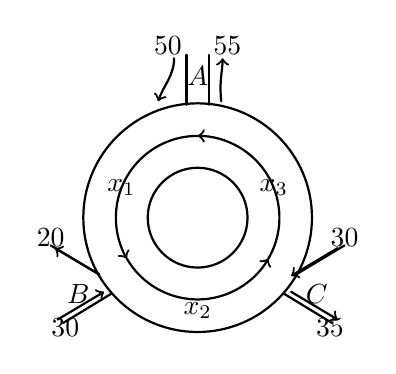
\begin{tikzpicture}[line cap=round,line join=round,scale=0.88]
  % 环岛外缘与中心圆岛
  \draw[thick] (0,0) circle (1.65);
  \draw[thick] (0,0) circle (0.72);

  % 三处外接道路
  \draw[thick] (-0.16,1.63)--(-0.16,2.35);
  \draw[thick] (0.16,1.63)--(0.16,2.35);
  \draw[thick] (-1.42,-0.82)--(-2.12,-0.40);
  \draw[thick] (-1.25,-1.10)--(-1.94,-1.52);
  \draw[thick] (1.42,-0.82)--(2.12,-0.40);
  \draw[thick] (1.25,-1.10)--(1.94,-1.52);

  % 环岛内部方向：A -> B -> C -> A
  \draw[->,thick] (90:1.18) arc (90:210:1.18);
  \draw[->,thick] (210:1.18) arc (210:330:1.18);
  \draw[->,thick] (330:1.18) arc (330:450:1.18);
  \node at (-1.10,0.43) {$x_1$};
  \node at (0,-1.34) {$x_2$};
  \node at (1.10,0.43) {$x_3$};

  % 路口 A：流入 50，流出 55
  \draw[->,thick] (-0.34,2.30) .. controls (-0.34,2.05) and (-0.49,1.91) .. (-0.57,1.68);
  \draw[->,thick] (0.34,1.68) .. controls (0.31,1.98) and (0.36,2.12) .. (0.36,2.30);
  \node at (-0.43,2.48) {$50$};
  \node at (0.43,2.48) {$55$};
  \node[above] at (0,1.76) {$A$};

  % 路口 B：流入 30，流出 20
  \draw[->,thick] (-1.42,-0.82)--(-2.06,-0.44);
  \draw[->,thick] (-2.02,-1.47)--(-1.35,-1.07);
  \node at (-2.12,-0.29) {$20$};
  \node at (-1.91,-1.59) {$30$};
  \node[below left] at (-1.42,-0.82) {$B$};

  % 路口 C：流入 30，流出 35
  \draw[->,thick] (2.02,-0.44)--(1.35,-0.84);
  \draw[->,thick] (1.35,-1.07)--(2.02,-1.47);
  \node at (2.12,-0.29) {$30$};
  \node at (1.91,-1.59) {$35$};
  \node[below right] at (1.42,-0.82) {$C$};
\end{tikzpicture}
\end{center}
\nopagebreak[4]
（A）$x_1>x_2>x_3$　　（B）$x_1>x_3>x_2$

（C）$x_2>x_3>x_1$　　（D）$x_3>x_2>x_1$

\end{question}
\gkpart{二、填空题}

\begin{gktip}
第9—14题位于固定 PDF 第1页（印刷页280）；同页的第15—17题属于下节解答题。
\end{gktip}

\begin{question}
\gkti{9}$\displaystyle\lim_{x\to-1}\dfrac{x^2+3x+2}{x^2-1}$ 的值等于\gkblank{}。

\end{question}
\begin{question}
\gkti{10}在 $\left(\sqrt{x}-\dfrac2x\right)^7$ 的展开式中，$x^2$ 的系数为\gkblank{}。（用数字作答）

\end{question}
\begin{question}
\gkti{11}若三点 $A(2,2)$、$B(a,0)$、$C(0,b)$（$ab\ne0$）共线，则 $\dfrac1a+\dfrac1b$ 的值等于\gkblank{}。

\end{question}
\begin{question}
\gkti{12}在 $\triangle ABC$ 中，若 $\sin A:\sin B:\sin C=5:7:8$，则 $\angle B$ 的大小是\gkblank{}。

\end{question}
\begin{question}
\gkti{13}已知点 $P(x,y)$ 的坐标满足条件
\nopagebreak[4]
\[
\begin{cases}
x+y\le 4,\\
y\ge x,\\
x\ge 1,
\end{cases}
\]
点 $O$ 为坐标原点，那么 $|PO|$ 的最小值等于\gkblank{}，最大值等于\gkblank{}。

\end{question}
\begin{question}
\gkti{14}已知 $A,B,C$ 三点在球心为 $O$、半径为 $R$ 的球面上，$AC\perp BC$，且 $AB=R$，那么 $A,B$ 两点的球面距离为\gkblank{}，球心到平面 $ABC$ 的距离为\gkblank{}。

\end{question}
\gkpart{三、解答题}

\begin{question}
\gkti{15}已知函数
\nopagebreak[4]
\[
f(x)=\frac{1-\sqrt2\sin\left(2x-\frac\pi4\right)}{\cos x}.
\]

（1） 求 $f(x)$ 的定义域；

（2） 设 $\alpha$ 是第四象限的角，且 $\tan\alpha=-\dfrac43$，求 $f(\alpha)$ 的值。

\Needspace{0.4\textheight}
\end{question}
\begin{question}
\gkti{16}已知函数 $f(x)=ax^3+bx^2+cx$ 在点 $x_0$ 处取得极大值5，其导函数 $y=f'(x)$ 的图象经过点 $(1,0),(2,0)$，如图所示，求：

（1） $x_0$ 的值；

（2） $a,b,c$ 的值。
\nopagebreak[4]
\begin{center}% Q16: 按固定候选 PDF 第1页（印刷页280）的示意图重绘；曲线仅表达向上开口与零点。
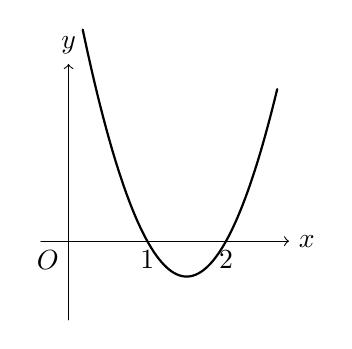
\begin{tikzpicture}[line cap=round,line join=round,scale=1.0]
  \draw[->] (-0.35,0)--(2.8,0) node[right] {$x$};
  \draw[->] (0,-1.0)--(0,2.25) node[above] {$y$};
  \draw[thick,domain=0.18:2.65,samples=80]
    plot (\x,{1.8*(\x-1)*(\x-2)});
  \node[below left] at (0,0) {$O$};
  \node[below] at (1,0) {$1$};
  \node[below] at (2,0) {$2$};
\end{tikzpicture}
\end{center}
\nopagebreak[4]
\Needspace{0.4\textheight}
\end{question}
\begin{question}
\gkti{17}如图，在底面为平行四边形的四棱锥 $P-ABCD$ 中，$AB\perp AC$，$PA\perp$ 平面 $ABCD$，且 $PA=AB$，点 $E$ 是 $PD$ 的中点。

（1） 求证：$AC\perp PB$；

（2） 求证：$PB\parallel$ 平面 $AEC$；

（3） 求二面角 $E-AC-B$ 的大小。
\nopagebreak[4]
\begin{center}% Q17: 按固定候选 PDF 第1页（印刷页280）重绘；保持原图标注与虚实关系，非比例图。
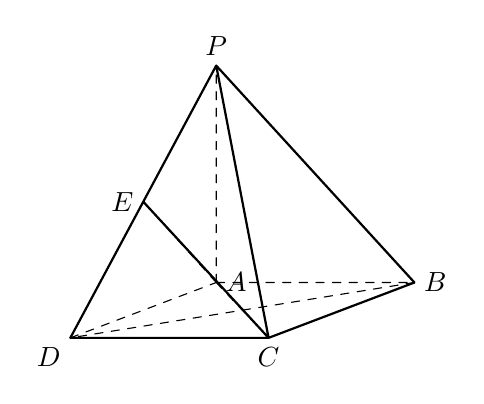
\begin{tikzpicture}[line cap=round,line join=round,scale=0.95]
  \coordinate (A) at (0,0);
  \coordinate (B) at (2.65,0);
  \coordinate (C) at (0.70,-0.74);
  \coordinate (D) at (-1.95,-0.74);
  \coordinate (P) at (0,2.90);
  \coordinate (E) at (-0.975,1.08);

  % 隐藏的底面边、底面对角线、PA 及题图辅助线
  \draw[dashed] (A)--(B) (B)--(D) (D)--(A) (A)--(C) (A)--(P) (A)--(E);
  % 可见棱与题图中的线段 EC
  \draw[thick] (B)--(C) (C)--(D) (P)--(B) (P)--(C) (P)--(D) (E)--(C);

  \node[above] at (P) {$P$};
  \node[right] at (A) {$A$};
  \node[right] at (B) {$B$};
  \node[below] at (C) {$C$};
  \node[below left] at (D) {$D$};
  \node[left] at (E) {$E$};
\end{tikzpicture}
\end{center}
\nopagebreak[4]
\begin{gktip}
以下第18—20题位于固定 PDF 第2页（印刷页281）。
\end{gktip}

\end{question}
\begin{question}
\gkti{18}某公司招聘员工，指定三门考试课程，有两种考试方案。

方案一：考试三门课程，至少有两门及格为考试通过；

方案二：在三门课程中，随机选取两门，这两门都及格为考试通过。

假设某应聘者对三门指定课程考试及格的概率分别是 $a,b,c$，且三门课程考试是否及格相互之间没有影响。

（1） 分别求该应聘者用方案一和方案二时考试通过的概率；

（2） 试比较该应聘者在上述两种方案下考试通过的概率的大小。（说明理由）

\end{question}
\begin{question}
\gkti{19}已知点 $M(-2,0)$、$N(2,0)$，动点 $P$ 满足条件 $|PM|-|PN|=2\sqrt2$。记动点 $P$ 的轨迹为 $W$。

（1） 求 $W$ 的方程；

（2） 若 $A,B$ 是 $W$ 上的不同两点，$O$ 是坐标原点，求 $\overrightarrow{OA}\cdot\overrightarrow{OB}$ 的最小值。

\end{question}
\begin{question}
\gkti{20}在数列 $\{a_n\}$ 中，若 $a_1,a_2$ 是正整数，且
\nopagebreak[4]
\[
a_n=|a_{n-1}-a_{n-2}|,\quad n=3,4,5,\ldots,
\]
则称 $\{a_n\}$ 为“绝对差数列”。

（1） 举出一个前五项不为零的“绝对差数列”（只要求写出前十项）；

\Needspace{5\baselineskip}
（2） 若“绝对差数列”$\{a_n\}$ 中 $a_{20}=3$、$a_{21}=0$，数列 $\{b_n\}$ 满足
\nopagebreak[4]
\[
b_n=a_n+a_{n+1}+a_{n+2},\quad n=1,2,3,\ldots,
\]
分别判断当 $n\to\infty$ 时，$a_n$ 与 $b_n$ 的极限是否存在；如果存在，求出其极限值；

（3） 证明：任何“绝对差数列”中总含有无穷多个为零的项。

\end{question}